
\renewcommand{\EntradaBibtex}{MarcoNuno_ReporteTecnico2024}

\begin{frame}{\citetitle{\EntradaBibtex}$^*$ (1)}
\begin{block}{Motivación} 
Es necesario automatizar el proceso de evaluación a nivel estatal de estudiantes de nivel medio superior
\end{block} 

\begin{itemize}
\item Se tuvo acceso a un repositorio de 6000 imágenes de digitalizaciones de examenes
\item Detectar los reactivos asignados de manera exacta (con el mínimo de errores) y generar un Excel con dicha información
\item Problemas: Variación en la iluminación, errores en el escaneo, forma de rellenar el circulo por parte de los estudiantes, etc.
\item Estos reactivos alimentan a otro sistema para obtener el resultado de la evaluación
\end{itemize}

\footfullcite*{\EntradaBibtex}
\end{frame}


\begin{frame}{\citetitle{\EntradaBibtex} (2)}
\begin{columns}

% Column 1
\column{.75\linewidth}
\begin{itemize}
\item Detectar rectangulos contenedores. Identificador (Superior) y Respuestas (Inferior)
\item Para los IDs:
\begin{itemize}
\item Se analiza por filas para obtener el ID
\item Opciones para cada fila del ID: 0-9, en blanco (X) o múltiple (M)
\item 4607 para el exámen mostrado
\end{itemize}
\item Para las respuestas:
\begin{itemize}
\item Deliminar una rejilla en donde se infieren están los aciertos.
\item Opciones para el acierto: A/B/C/D, en blanco (X) o múltiple (M)
\end{itemize}
\end{itemize}
\column{.25\linewidth}
	\begin{center}
	%\begin{tabular}{cc}
		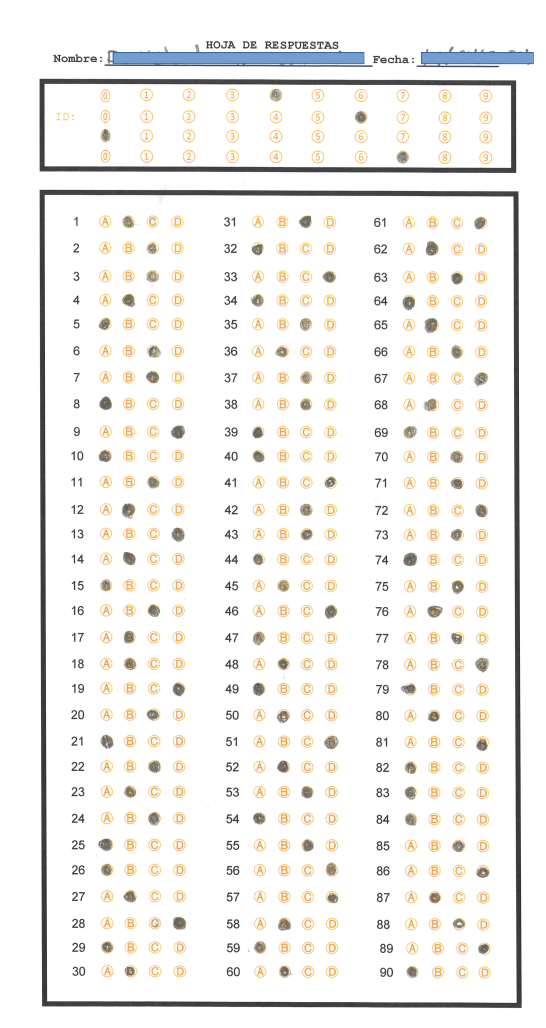
\includegraphics[width=0.90\linewidth]{2024_ProyectoCalificadorExamenes/figs/ExamenES1.png}
		%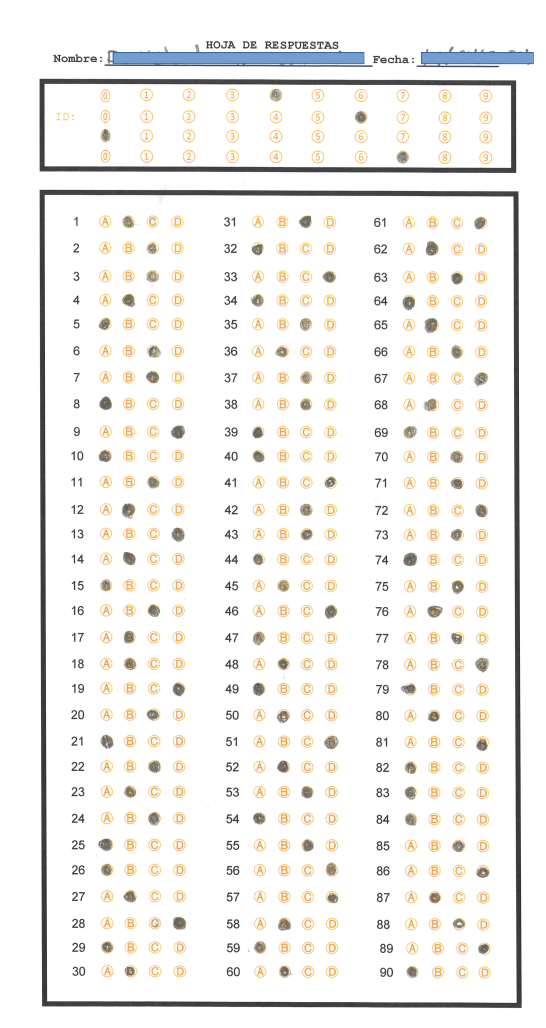
\includegraphics[width=0.20\linewidth]{2024_ProyectoCalificadorExamenes/figs/ExamenES1.png} \\
	%\end{tabular}
\end{center}

\end{columns}

\end{frame}


\begin{frame}{\citetitle{\EntradaBibtex} (3)}
Problemas Detectados
\begin{center}
	\begin{tabular}{ccc}
		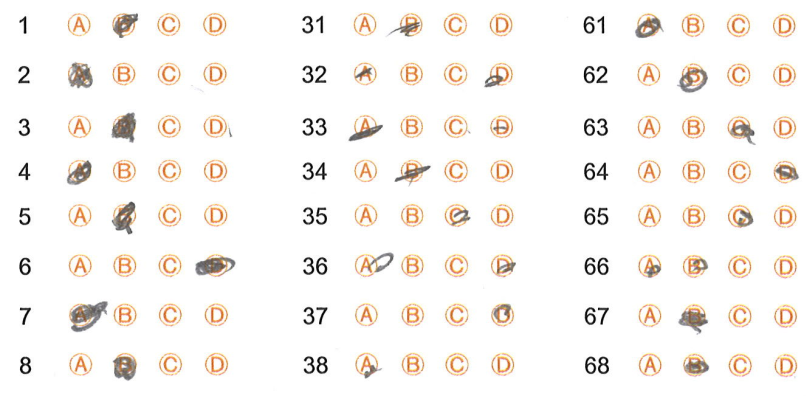
\includegraphics[width=0.35\linewidth]{2024_ProyectoCalificadorExamenes/figs/CasoFlojera.png}&
		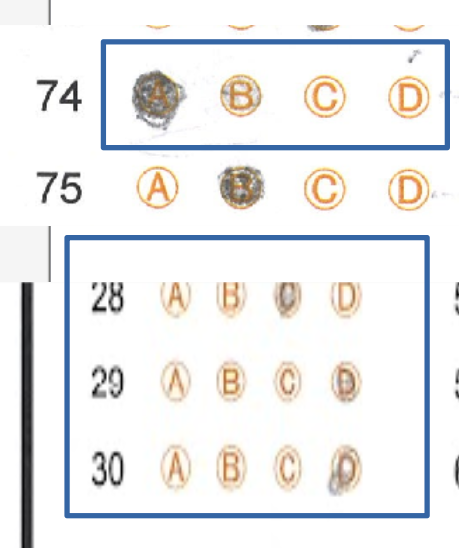
\includegraphics[width=0.10\linewidth]{2024_ProyectoCalificadorExamenes/figs/CasosBorrosos.png} &
		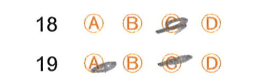
\includegraphics[width=0.15\linewidth]{2024_ProyectoCalificadorExamenes/figs/RespuestaMultiple.png} \\
		Circulos no completos & Borrado de respuesta & Respuesta Multiple \\ 

	\end{tabular}
\end{center}
Estado:
\begin{itemize}
\item Se está evaluando la precisión del sistema (Se estima por arriba del 95\%)
\item Se generó una interfaz para seleccionar carpetas de examenes. Organizados por centro de institucion y semestre (2do, 4to y 6to) y se genera el archivo de Excel con las respuestas
\end{itemize}



\end{frame}

